\documentclass{beamer}
\usepackage[utf8]{inputenc}

\usetheme{Madrid}
\usecolortheme{default}
\usepackage{amsmath,amssymb,amsfonts,amsthm}
\usepackage{txfonts}
\usepackage{tkz-euclide}
\usepackage{listings}
\usepackage{adjustbox}
\usepackage{array}
\usepackage{tabularx}
\usepackage{gvv}
\usepackage{lmodern}
\usepackage{circuitikz}
\usepackage{tikz}
\usepackage{graphicx}
\usepackage{caption}
\captionsetup{labelformat=empty}  % removes "Figure:"


\setbeamertemplate{page number in head/foot}[totalframenumber]

\usepackage{tcolorbox}
\tcbuselibrary{minted,breakable,xparse,skins}



\definecolor{bg}{gray}{0.95}
\DeclareTCBListing{mintedbox}{O{}m!O{}}{%
	breakable=true,
	listing engine=minted,
	listing only,
	minted language=#2,
	minted style=default,
	minted options={%
		linenos,
		gobble=0,
		breaklines=true,
		breakafter=,,
		fontsize=\small,
		numbersep=8pt,
		#1},
	boxsep=0pt,
	left skip=0pt,
	right skip=0pt,
	left=25pt,
	right=0pt,
	top=3pt,
	bottom=3pt,
	arc=5pt,
	leftrule=0pt,
	rightrule=0pt,
	bottomrule=2pt,
	toprule=2pt,
	colback=bg,
	colframe=orange!70,
	enhanced,
	overlay={%
		\begin{tcbclipinterior}
			\fill[orange!20!white] (frame.south west) rectangle ([xshift=20pt]frame.north west);
	\end{tcbclipinterior}},
	#3,
}
\lstset{
	language=C,
	basicstyle=\ttfamily\small,
	keywordstyle=\color{blue},
	stringstyle=\color{orange},
	commentstyle=\color{green!60!black},
	numbers=left,
	numberstyle=\tiny\color{gray},
	breaklines=true,
	showstringspaces=false,
}
\begin{document}

\title 
{1.8.23}
\date{oct 4,2025}

\author 
{ADUDOTLA SRIVIDYA - EE25BTECH11006}
\graphicspath{./figs}


\frame{\titlepage}
\begin{frame}{Question}
If the point $\textbf{A}(2,-4)$ is equidistant from $\textbf{P}(3,8)$ and $\textbf{Q}(-10,y)$, find the values of $y$.
 Also find distance $\vec{PQ}$.

 \begin{table}[H]
\centering
\begin{tabular}{|c|c|c|}
\hline
\textbf{Symbol} & \textbf{Value} & \textbf{Description} \\
\hline
$A$ & $\myvec{2 \\ -4}$ & equidistant point \\
\hline
$P$ & $\myvec{3 \\ 8}$ & First point \\
\hline
$Q$ & $\myvec{-10 \\ y}$ & Second point \\
\hline
\end{tabular}
\caption{Parameters for the problem}
\end{table}
\end{frame}

\begin{frame}{Theoretical Solution}
Since $\vec{A}$ is equidistant from $\vec{P}$ and $\vec{Q}$,

\begin{align}
    \norm{\myvec{\vec{A} - \vec{P}}} = \norm{\myvec{\vec{A} - \vec{Q}}}
\end{align}

\begin{align}
     \norm{\myvec{\vec{A} - \vec{P}}}^2 = \norm{\myvec{\vec{A} - \vec{Q}}}^2
\end{align}

\begin{align}
    {(\vec{A} - \vec{P})}^\top (\vec{A} - \vec{P}) \, &= \, {(\vec{A} - \vec{Q})}^\top (\vec{A} - \vec{Q})
\end{align}

\begin{align}
 {||\vec{A}||}^2 \, - \, 2\vec{A}^\top\vec{P} \, + \, {||\vec{P}||}^2 \, = \, {||\vec{A}||}^2 \, - \, 2\vec{A}^\top\vec{Q} \, + \, {||\vec{Q}||}^2
\end{align}

\end{frame}

\begin{frame}
\begin{align}
    {(\vec{P} - \vec{Q})}^\top \vec{A} \, &= \, \frac{{||\vec{P}||}^2\, - \, {||\vec{Q}||}^2}{2}
\end{align}

\begin{align}
    \myvec{3-(-10)\\8-y}^\top\myvec{2\\-4}\, = \, \frac{73-(-10)^2 -y^2}{2}
\end{align}

\begin{align}
    y^2 +8y + 15 = 0
\end{align}

Therefore,
\begin{align}
    y \, = -5 , -3
\end{align}

\begin{align}
   \vec{Q_1} = \myvec{-10 \\ -5}, \quad
   \vec{Q_2} = \myvec{-10 \\ -3}
\end{align}
\end{frame}

\begin{frame}{Distance}
\begin{align}
    \norm{\myvec{\vec{P} - \vec{Q_1}}} &= \left\|\myvec{3\\8} - \myvec{-10\\-5}\right\| \\
    &= \left\|\myvec{13\\13}\right\| \\
    &= 13\sqrt{2}
\end{align}

\begin{align}
    \norm{\myvec{\vec{P} - \vec{Q_2}}} &= \left\|\myvec{3\\8} - \myvec{-10\\-3}\right\| \\
    &= \left\|\myvec{13\\11}\right\| \\
    &= \sqrt{290}
\end{align}

\end{frame}

\begin{frame}[fragile]
\frametitle{Python,C,Python+C codes}
codes permalink
\end{frame}

\begin{frame}{Plot}
   \begin{figure}[H]
\centering
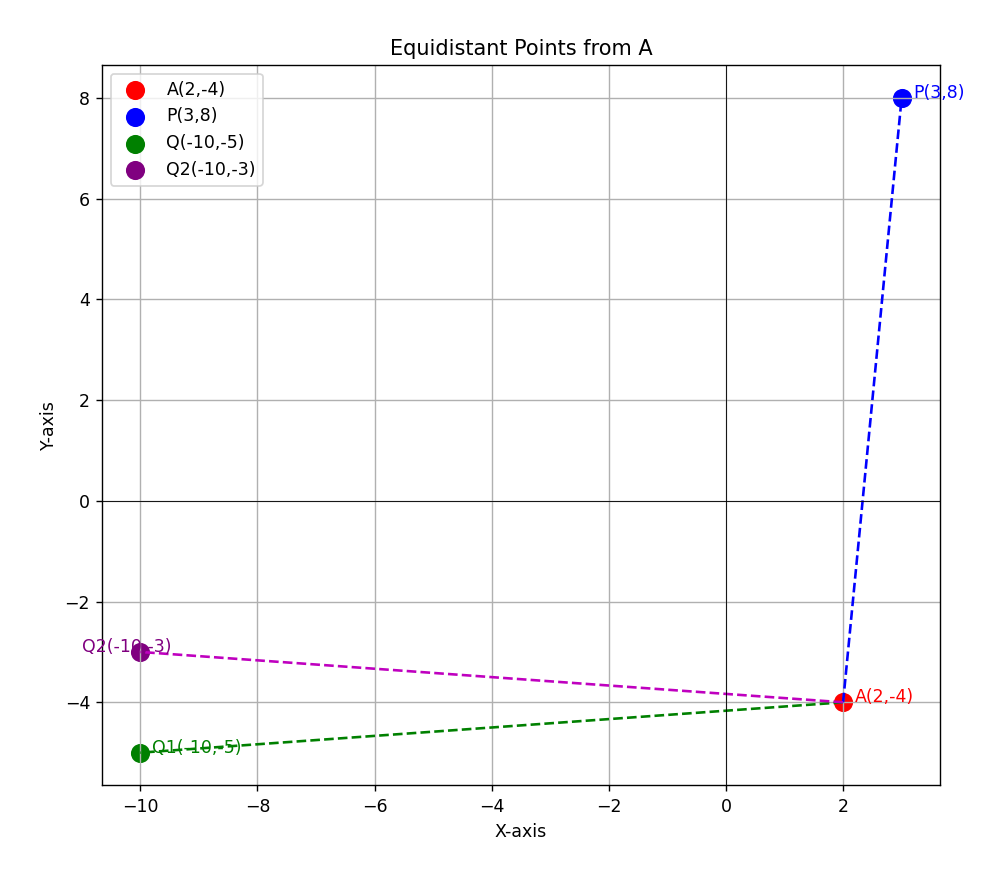
\includegraphics[width=0.6\columnwidth]{../beamer/figs/fig1.png}
 \caption*{Equidistant Points from $\vec{A}$}
\label{fig:graph.png}
\end{figure}
\end{frame}

\end{document}